% witness: synthetic (the `\halign`s that stay the SVG matrix: tikz's `align=` lines, tikz.code.tex:4253, and a matrix
%          in a picture nested in a node's text, pgfmodulematrix.code.tex:191-193; amsmath's own alignments beside them)
% oracle:  pdflatex 0 errors: "first line / second line / third", "Top / mid", the pmatrix, the cases, "outer p q r s"
% engines: rust INT081AB and HALIGNINT byte-identical
% expect:  0 errors; the `align=` lines and the nested matrix SVG matrices, the pmatrix and cases XMArrays
% status:  GREEN (HALIGNINT, OXIDIZED_DESIGN_DIVERGENCES #1167)
\documentclass{article}
\usepackage{tikz}
\usepackage{amsmath}
\usetikzlibrary{matrix}
\begin{document}
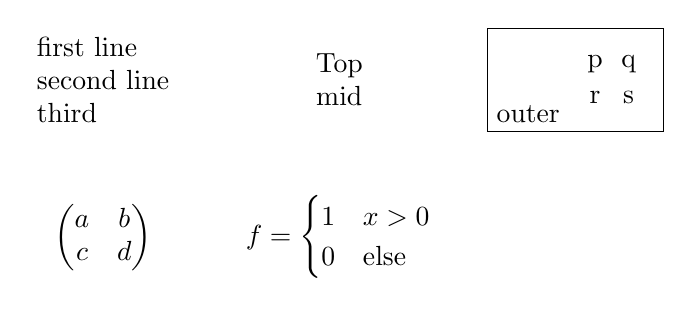
\begin{tikzpicture}
\node[align=left] {first line\\ second line\\ third};
\node[align=center] at (3,0) {Top\\ mid};
\node at (0,-2) {$\begin{pmatrix} a & b\\ c & d\end{pmatrix}$};
\node at (3,-2) {$f=\begin{cases} 1 & x>0\\ 0 & \text{else}\end{cases}$};
\node[draw] at (6,0) {outer \tikz{\matrix[matrix of nodes]{p & q\\ r & s\\};}};
\end{tikzpicture}
\end{document}
